\documentclass[11pt]{article}

% ------------------------- Packages -------------------------
\usepackage[margin=1in]{geometry}
\usepackage{graphicx}
\usepackage{amsmath, amssymb}
\DeclareMathOperator*{\argmin}{arg\,min}
\usepackage{hyperref}
\usepackage{xcolor}
\usepackage{listings}
\usepackage{caption}
\usepackage{subcaption}
\usepackage{enumitem}

% ------------------------- Listings style -------------------------
\lstdefinestyle{pystyle}{
    language=Python,
    basicstyle=\ttfamily\footnotesize,
    keywordstyle=\color{blue!70!black}\bfseries,
    commentstyle=\color{gray}\itshape,
    stringstyle=\color{orange!70!black},
    numbers=left,
    numberstyle=\tiny\color{gray},
    stepnumber=1,
    numbersep=8pt,
    frame=single,
    breaklines=true,
    breakatwhitespace=false,
    showstringspaces=false,
    tabsize=4,
    captionpos=b,
}
\lstset{style=pystyle}

\title{Reproducing the Core Ideas of MERIT: \\
       A Small-Scale PyTorch Demo for Multi-Domain RAW Image Translation}
\author{
    Erfan Tabatabaei \\
    \small Digital Image Processing - Final Project \\
    \small Dr. Ghiasi \\
    \small \today
}
\date{}

\begin{document}
\maketitle
\thispagestyle{empty}
\newpage

\begin{abstract}
This report documents a small-scale PyTorch reimplementation of the core
ideas from \emph{MERIT: Multi-domain Efficient RAW Image Translation}
\cite{merit2026}. The original paper introduces a single generator,
conditioned on a learned style embedding, capable of translating RAW
images between an arbitrary number of camera sensor domains without
requiring paired training data. Because real multi-camera RAW datasets
(e.g., the paper's MDRAW benchmark) were not available for this exercise,
this project instead builds a fully synthetic pipeline: two ``camera
domains'' are simulated with distinct spectral tints and Poisson-Gaussian
noise profiles, a scaled-down generator and style encoder are trained
under an unpaired, cycle-consistency-based objective, and the result is
evaluated with the two of the metrics used in the paper (MAE, PSNR).
This report summarizes the original method,
describes the demo's architecture and training procedure in detail,
and explicitly enumerates every point where the demo simplifies or
deviates from the full MERIT design.
\end{abstract}
\newpage

\tableofcontents
\newpage

% =====================================================================
\section{Introduction}
% =====================================================================

RAW images captured by different camera sensors differ substantially in
color response, dynamic range, and noise characteristics, even when
photographing the same scene. This domain shift, rooted in each sensor's
distinct spectral response function $R_c(\lambda)$, forces practitioners
to either train a separate downstream model per camera or translate RAW
images into a common target domain before further processing. MERIT
\cite{merit2026} proposes a single, unified generator that performs this
RAW-to-RAW (RAW2RAW) translation across an arbitrary number of camera
domains, replacing the one-to-one translators used by prior work.

The goal of this project is \textbf{not} to reproduce MERIT's reported
benchmark numbers -- doing so would require the paper's MDRAW dataset and
full training budget (200{,}000 iterations on an NVIDIA H200 GPU) -- but
to build a working, inspectable implementation of the paper's central
mechanisms:
\begin{itemize}[nosep]
    \item a content-independent style encoder $E$,
    \item a style-conditioned generator $G$ with a multi-scale
          large-kernel-attention (MS-LKA) module,
    \item an unpaired training loop using cycle-consistency and
          style-reconstruction losses,
    \item brightness-based reference selection at inference time, and
    \item the paper's two metrics (MAE, PSNR) evaluation protocol.
\end{itemize}

% =====================================================================
\section{Background: The MERIT Framework}
% =====================================================================

This section summarizes the relevant parts of \cite{merit2026} that the
demo is based on.

\subsection{Problem Formulation}
Let $\mathcal{X}$ be the set of RAW images and $\mathcal{Y}$ the set of
camera domains. Given an image $I^a \in \mathcal{X}$ from source domain
$a \in \mathcal{Y}$, MERIT trains a single generator $G$ that can produce
the corresponding image $\hat{I}^b$ in any target domain
$b \in \mathcal{Y} \setminus \{a\}$:
\begin{equation}
    \hat{I}^b = G(I^a, s_b), \qquad s_b = E(I^b),
\end{equation}
where $E$ is a learnable \emph{style encoder} that extracts a
domain-specific, content-independent embedding $s_b$ from a reference
image $I^b$ of the target domain.

\subsection{Architecture (Paper)}
The paper's architecture (Fig.~2) has three components:
\begin{enumerate}[nosep]
    \item \textbf{Style Encoder $E$}: patchifies the input image, prepends
          a learnable style token, and applies self-attention
          (query/key/value) over the resulting tokens to produce $s_b$.
    \item \textbf{Generator $G$}: a convolutional encoder--decoder with a
          \emph{Transformer block} at the bottleneck and a
          \emph{Multi-Scale Large Kernel Attention (MS-LKA)} module on
          the upsampling path.
    \item \textbf{Discriminator $D$}: a patch-based discriminator that
          classifies real vs.\ generated patches and aggregates the
          patch-level decisions via majority voting.
\end{enumerate}

\subsection{Sensor-Aware Noise Modeling (SANM)}
RAW sensor noise is modeled as Poisson-Gaussian:
\begin{equation}
    \mathrm{Var}(x) = \alpha \cdot z + \beta,
\end{equation}
where $z$ is the true scene intensity, $\alpha$ is the signal-dependent
(shot) noise coefficient, and $\beta$ is the signal-independent (read)
noise variance. The paper introduces a differentiable, histogram-based
noise loss $\mathcal{L}_{\text{noise}}$ that matches the noise profile of
generated images to that of the target domain, estimated from
low-texture (flat) image patches identified via a Sobel gradient filter.

\subsection{Multi-Scale Large Kernel Attention (MS-LKA)}
MS-LKA (Sec.~2.3 of \cite{merit2026}) replaces expensive full
self-attention with three parallel depthwise convolutions at dilation
rates $\{1, 4, 9\}$, fused via a $1\times1$ convolution, and then
re-weighted channel-wise by a style-conditioned gate:
\begin{align}
    F_{\text{concat}} &= \mathrm{Conv}_{1\times1}([F_1; F_2; F_3]), \\
    F_{\text{out}} &= A_s \odot F_{\text{concat}},
\end{align}
where $A_s \in \mathbb{R}^C$ is produced from the style embedding $s$ by
a lightweight feed-forward network.

\subsection{Loss Functions}
The full MERIT objective combines five terms:
\begin{equation}
    \mathcal{L}_{\text{total}} = \lambda_1 \mathcal{L}_{\text{noise}}
        + \lambda_2 \mathcal{L}_{\text{adv}}^D
        + \lambda_3 \mathcal{L}_{\text{adv}}^G
        + \lambda_4 \mathcal{L}_{\text{cycle-L1}}
        + \lambda_5 \mathcal{L}_{\text{cycle-SSIM}}.
\end{equation}

\subsection{Datasets and Metrics}
The paper evaluates on the public RAW-to-RAW Mapping Dataset (Samsung
Galaxy S9 / iPhone X, 392 unpaired + 115 paired images) \cite{afifi2021}
and its own MDRAW dataset (five camera sensors, 519 unpaired + 285
paired images), using four metrics: MAE, PSNR, SSIM, and a symmetric,
histogram-based KL divergence.

% =====================================================================
\section{Project Structure}
% =====================================================================

\begin{verbatim}
dip_project/
|-- MERIT.pdf
|-- README.md
`-- src/
    |-- data_generator.py      (synthetic RAW domain generator)
    |-- data_preprocessing.py  (linearization + Bayer packing)
    |-- model.py               (StyleEncoder, MS-LKA, Generator)
    |-- train.py               (unsupervised training loop)
    |-- evaluate.py            (MAE/PSNR + plotting)
    `-- main.py                (end-to-end entry point)
\end{verbatim}

Table~\ref{tab:mapping} maps each file to the paper section it
implements.

\begin{table}[h]
\centering
\caption{File-to-paper mapping.}
\label{tab:mapping}
\begin{tabular}{ll}
\hline
\textbf{File} & \textbf{Paper section} \\
\hline
\texttt{data\_generator.py} & Sec.~1 (image formation, Eq.~1),
                              Sec.~2.2 (Poisson-Gaussian noise, Eq.~2) \\
\texttt{data\_preprocessing.py} & Sec.~7.1 (linearization, RGGB packing) \\
\texttt{model.py} & Sec.~2.1 (Style Encoder \& Generator),
                     Sec.~2.3 (MS-LKA) \\
\texttt{train.py} & Sec.~2.4 (loss functions -- subset, see
                     Sec.~\ref{sec:deviations}) \\
\texttt{evaluate.py} & Sec.~8 of supplementary (MAE, PSNR) \\
\texttt{main.py} & Sec.~3 (brightness-based reference selection) \\
\hline
\end{tabular}
\end{table}

% =====================================================================
\section{Synthetic Data Generation}
% =====================================================================

Since dataset was so big and we didnt have enough memory, two synthetic camera
domains are constructed with a \texttt{DomainProfile}: a per-RGGB-channel
gain vector (standing in for the sensor's spectral response $R_c(\lambda)$)
and a pair of Poisson-Gaussian noise coefficients $(\alpha, \beta)$
matching Eq.~2 of the paper. Each domain is seeded deterministically for
reproducibility.

\begin{itemize}[nosep]
    \item \texttt{\_base\_scene}: generates smooth, low-frequency random
          content standing in for real-world scene radiance $S(x,\lambda)$.
    \item \texttt{render\_domain\_raw}: applies a domain's tint, injects
          Poisson-Gaussian noise, and re-embeds the result into
          $[\text{black\_level}, \text{white\_level}]$.
    \item \texttt{sample\_unpaired\_batch}: draws independent scenes per
          domain call -- used for \emph{training}, matching the paper's
          unpaired setting.
    \item \texttt{sample\_paired\_batch}: renders the \emph{same} scene
          through two domains -- used only for \emph{evaluation}, since a
          real ground truth is required to compute MAE/PSNR.
\end{itemize}

% =====================================================================
\section{Preprocessing}
% =====================================================================

\texttt{RawPreprocessor} mirrors the first stage of a real RAW pipeline:
\begin{equation}
    I_{\text{linear}} = \mathrm{clip}\!\left(
        \frac{I_{\text{raw}} - \text{black\_level}}
             {\text{white\_level} - \text{black\_level}},\ 0, 1
    \right),
\end{equation}
the exact inverse of the range remapping performed by
\texttt{render\_domain\_raw}. It also implements lossless packing between
a single-channel mosaiced Bayer image $(B,1,H,W)$ and the 4-channel
packed RGGB representation $(B,4,H/2,W/2)$ used everywhere else in the
pipeline, following the RGGB tiling
$\begin{pmatrix} R & G_r \\ G_b & B \end{pmatrix}$.

% =====================================================================
\section{Model Architecture}
% =====================================================================

\subsection{Style Encoder}
A four-layer strided convolutional stack (channels
$4 \to 32 \to 64 \to 128 \to 128$, each halving spatial resolution)
followed by global average pooling and a linear projection to a
64-dimensional style vector:
\begin{equation}
    (B,4,128,128) \xrightarrow{\text{4 conv layers}} (B,128,8,8)
    \xrightarrow{\text{GAP}} (B,128) \xrightarrow{\text{Linear}} (B,64).
\end{equation}
Global average pooling is the critical step that discards spatial
content, yielding an embedding that is (approximately) content
independent, as intended by the paper.

\subsection{MS-LKA Module}
Implemented faithfully to Sec.~2.3 of the paper: three parallel
depthwise convolutions at dilation rates $\{1,4,9\}$ (effective receptive
fields of $5\times5$, $17\times17$, and $37\times37$ for a $5\times5$
kernel), fused with a $1\times1$ convolution, then gated channel-wise by
a sigmoid MLP conditioned on the style vector, with a residual
connection.

\subsection{Generator}
A small U-Net: a full-resolution stem, two downsampling stages
($128\!\to\!64\!\to\!32$), a bottleneck, and two upsampling stages with
skip connections and an MS-LKA refinement at each stage. The final
$1\times1$ convolution projects back to 4 channels, followed by a
sigmoid to keep outputs in $[0,1]$.

\subsection{Deviations from the Paper's Architecture}
\label{sec:arch-deviations}
\begin{table}[h]
\centering
\caption{Architectural simplifications made in this demo.}
\begin{tabular}{p{4.2cm}p{5cm}p{5cm}}
\hline
\textbf{Component} & \textbf{Paper (Fig.~2)} & \textbf{This demo} \\
\hline
Style Encoder & Patchify $\to$ tokens $\to$ self-attention
                (Q/K/V) over a learnable style token
              & Plain convolutional stack $+$ global average
                pooling $+$ linear layer \\
Generator bottleneck & Conv $\to$ \textbf{Transformer block}
                        $\to$ Conv
                      & Conv $\to$ Conv (no self-attention) \\
Generator upsampling path & MS-LKA & MS-LKA (implemented as in
                                      the paper) \\
Discriminator & Patch-based, majority-vote adversarial
                discriminator & Not implemented (see
                Sec.~\ref{sec:deviations}) \\
\hline
\end{tabular}
\end{table}

% =====================================================================
\section{Training Procedure}
% =====================================================================

Training follows the paper's \emph{unpaired} sampling strategy: at each
step, a batch of domain-A images and an independent batch of domain-B
images are drawn (no pixel alignment between them). For each source
image $I^a$ and a randomly chosen reference $I^b$:
\begin{align}
    s_b &= E(I^b), &
    \hat{I}^b &= G(I^a, s_b), \\
    s_a &= E(I^a), &
    \hat{I}^a &= G(\hat{I}^b, s_a).
\end{align}

Two losses are used:
\begin{align}
    \mathcal{L}_{\text{style}} &= \| E(\hat{I}^b) - s_b \|_1, \\
    \mathcal{L}_{\text{cycle}} &= \| I^a - \hat{I}^a \|_1.
\end{align}
\begin{equation}
    \mathcal{L}_{\text{total}} = \lambda_{\text{cycle}} \, \mathcal{L}_{\text{cycle}}
        + \lambda_{\text{style}} \, \mathcal{L}_{\text{style}},
    \qquad \lambda_{\text{cycle}} = 10,\ \lambda_{\text{style}} = 1.
\end{equation}

\subsection{Data Volume}
Because \texttt{sample\_unpaired\_batch} generates fresh random scenes on
every call rather than drawing from a fixed pool, there is no meaningful
notion of ``dataset size'' or ``epoch'' in this demo -- each of the
\texttt{steps} $\times$ \texttt{batch\_size} images seen during training
is unique. With the default configuration
(\texttt{steps=150}, \texttt{batch\_size=8}), the model observes
$150 \times 8 = 1{,}200$ domain-A images and $1{,}200$ domain-B images
over the course of training, none of which repeat.

\subsection{Observed Training Convergence}
\label{sec:training-run}
Table~\ref{tab:losscurve} reports the logged loss values from an actual
150-step training run. The total loss decreases steadily and roughly
monotonically, driven primarily by the cycle-consistency term (which
carries the larger weight, $\lambda_{\text{cycle}}=10$); the style
loss stays small and comparatively flat throughout training, consistent
with the style encoder converging quickly to a stable, mostly
content-independent embedding early on.

\begin{table}[h]
\centering
\caption{Logged training loss over 150 steps
         (\texttt{batch\_size=8}, \texttt{img\_size=128}, CPU).}
\label{tab:losscurve}
\begin{tabular}{ccccc}
\hline
Step & Total loss & Cycle loss ($\mathcal{L}_{\text{cycle}}$) & Style loss ($\mathcal{L}_{\text{style}}$) \\
\hline
1   & 2.1812 & 0.2175 & 0.0066 \\
25  & 1.2967 & 0.1290 & 0.0067 \\
50  & 1.1258 & 0.1120 & 0.0057 \\
75  & 0.9629 & 0.0957 & 0.0062 \\
100 & 0.8389 & 0.0833 & 0.0064 \\
125 & 0.7394 & 0.0734 & 0.0058 \\
150 & 0.6565 & 0.0651 & 0.0058 \\
\hline
\end{tabular}
\end{table}

Total loss dropped by roughly 70\% over the course of training
(from $2.18$ at step 1 to $0.66$ at step 150), with no signs of
divergence or instability -- a reasonable sanity check that the
cycle-consistency and style-reconstruction gradients are well-behaved
for this synthetic setup, even without an adversarial term.

\subsection{Deviations from the Paper's Training Objective}
\label{sec:deviations}
\begin{table}[h]
\centering
\caption{Loss-function and training simplifications.}
\begin{tabular}{p{4.5cm}p{4.5cm}p{4.5cm}}
\hline
\textbf{Element} & \textbf{Paper} & \textbf{This demo} \\
\hline
Adversarial loss ($\mathcal{L}_{\text{adv}}^{D}, \mathcal{L}_{\text{adv}}^{G}$)
    & Patch-based discriminator, majority-vote real/fake
    & \textbf{Not implemented} -- no discriminator \\
Noise loss ($\mathcal{L}_{\text{noise}}$)
    & Histogram-based, Sobel-filtered flat-patch noise
      profile matching
    & \textbf{Not implemented} \\
Cycle-consistency SSIM ($\mathcal{L}_{\text{cycle-SSIM}}$)
    & Included in full objective
    & \textbf{Not implemented}; only L1 cycle loss used \\
Training scale & 200{,}000 iterations, real camera data,
                 batch size 8, H200 GPU
               & 150 iterations (configurable), synthetic
                 data, batch size 8, CPU/GPU \\
\hline
\end{tabular}
\end{table}

% =====================================================================
\section{Inference: Brightness-Based Reference Selection}
% =====================================================================

At inference time, the paper selects the target-domain reference image
whose per-channel (RGGB) mean brightness vector is closest to the
source's, rather than choosing an arbitrary reference. This matters
because the style embedding is only \emph{approximately}
content-independent -- the paper notes it ``may still depend on some
characters (e.g., brightness)'' -- so an exposure-mismatched reference
can leak an unwanted brightness shift into the translation.

Formally, given a query image and a pool of $N$ candidate references,
\begin{equation}
    b(I) = \frac{1}{HW}\sum_{h,w} I(:,h,w) \in \mathbb{R}^4,
\end{equation}
\begin{equation}
    I^{\text{ref}} = \argmin_{I_i \in \text{pool}}
        \left\lVert b(I_{\text{query}}) - b(I_i) \right\rVert_2 .
\end{equation}
This is implemented in \texttt{select\_reference\_by\_brightness} using
\texttt{torch.cdist} over a pool of 16 candidate domain-B images.

\paragraph{Worked example (actual run).} For one query image, the
selection procedure produced the following per-channel (R, $G_r$,
$G_b$, B) brightness vectors:
\begin{align*}
    b(I_{\text{query}}) &= [0.4747,\ 0.5747,\ 0.3941,\ 0.3908] \\
    b(I^{\text{ref}})   &= [0.5307,\ 0.4619,\ 0.4678,\ 0.5289] \\
    b(\hat{I}^{b})       &= [0.4878,\ 0.5478,\ 0.4036,\ 0.4097]
\end{align*}
Notably, the translated output's brightness vector $b(\hat{I}^b)$ sits
much closer to the query's $b(I_{\text{query}})$ than to the selected
reference's $b(I^{\text{ref}})$ -- i.e., the generator did not simply
copy the reference's exposure onto the output. This is the expected
behavior: the style embedding is meant to carry the target domain's
color/noise character, while the source image's own brightness should
be substantially preserved through the skip connections in the
generator.

% =====================================================================
\section{Evaluation}
% =====================================================================

Four metrics are computed between the translated output and a paired
ground truth (obtained only for evaluation via
\texttt{sample\_paired\_batch}, and never used as the style reference,
to keep the evaluation honest):

\begin{align}
    \text{MAE} &= \frac{1}{N}\sum_i |I_p(i) - I_r(i)| \\
    \text{PSNR} &= 10 \log_{10}\!\left(\frac{L^2}{\text{MSE}}\right) \\
\end{align}

\textbf{Implementation note.} SSIM is computed with a uniform (box)
window rather than the paper's implied windowing, and the KL divergence
uses 64 histogram bins rather than the paper's 256 -- both simplifications
for speed and code brevity; see \texttt{evaluate.py}.

\subsection{Reference vs.\ Ground Truth}
It is worth stating explicitly, since it is easy to conflate the two:
the \textbf{style reference} (an unpaired, brightness-matched domain-B
image) is an \emph{input} to the model, used only to extract a style
embedding; the \textbf{ground truth} (a paired domain-B rendering of the
exact same synthetic scene as the source) is never seen by the model and
exists solely to score the output after the fact.

% =====================================================================
\section{Results}
% =====================================================================

\begin{table}[h]
\centering
\caption{Quantitative results on the synthetic two-domain demo. The
         untrained row uses all four metrics from an earlier sanity
         check; the trained row reflects the metrics actually reported
         by \texttt{evaluate.py} for this run (MAE, PSNR only).}
\label{tab:results}
\begin{tabular}{lcccc}
\hline
Setting & MAE $\downarrow$ & PSNR $\uparrow$ & SSIM $\uparrow$ & KL $\downarrow$ \\
\hline
Untrained (sanity check) & 0.2163 & 11.61 dB & 0.0995 & 3.1010 \\
Trained (150 steps)      & 0.2589 & 9.75 dB  & --     & --     \\
\hline
\end{tabular}
\end{table}

\paragraph{An honest reading of this result.} Somewhat counter-intuitively,
MAE and PSNR against the paired ground truth are \emph{worse} after
training than the untrained sanity check. This is a real, reported
result rather than an error, and is worth explaining rather than
hiding: the training objective used here
(Sec.~\ref{sec:deviations}, $\mathcal{L}_{\text{cycle}}$ and
$\mathcal{L}_{\text{style}}$ only) never directly supervises the model
against a specific paired target -- there is no term in the loss that
pulls $\hat{I}^b$ toward any particular ground-truth image, only toward
(a) being cycle-consistent with $I^a$ and (b) reproducing the style of
\emph{whichever} reference $I^b$ was randomly sampled that step. Since
the evaluation's ground truth and the brightness-matched reference are
different images (Sec.~9.1), nothing in this reduced loss set commits
the model to landing close to the ground truth pixel values -- unlike
the full MERIT objective, where the adversarial loss anchors outputs to
the realistic target-domain \emph{distribution} and
$\mathcal{L}_{\text{noise}}$ explicitly matches sensor statistics.
Without those terms, the model is free to converge toward \emph{a}
domain-B-like tint that satisfies cycle-consistency without necessarily
approaching the one specific paired sample used for scoring. This is
consistent with the loss curve in Table~\ref{tab:losscurve}, where
$\mathcal{L}_{\text{cycle}}$ and $\mathcal{L}_{\text{style}}$ both
decrease steadily -- the model \emph{is} learning to optimize what it
was actually told to optimize, it simply was not told to optimize
paired-image fidelity. This is a useful negative result: it isolates
exactly why the paper's adversarial and noise losses
(Sec.~\ref{sec:deviations}) are not optional extras but are load-bearing
for the paper's reported quality numbers (Tables~2--5 of
\cite{merit2026}).

\begin{figure}[h]
    \centering
    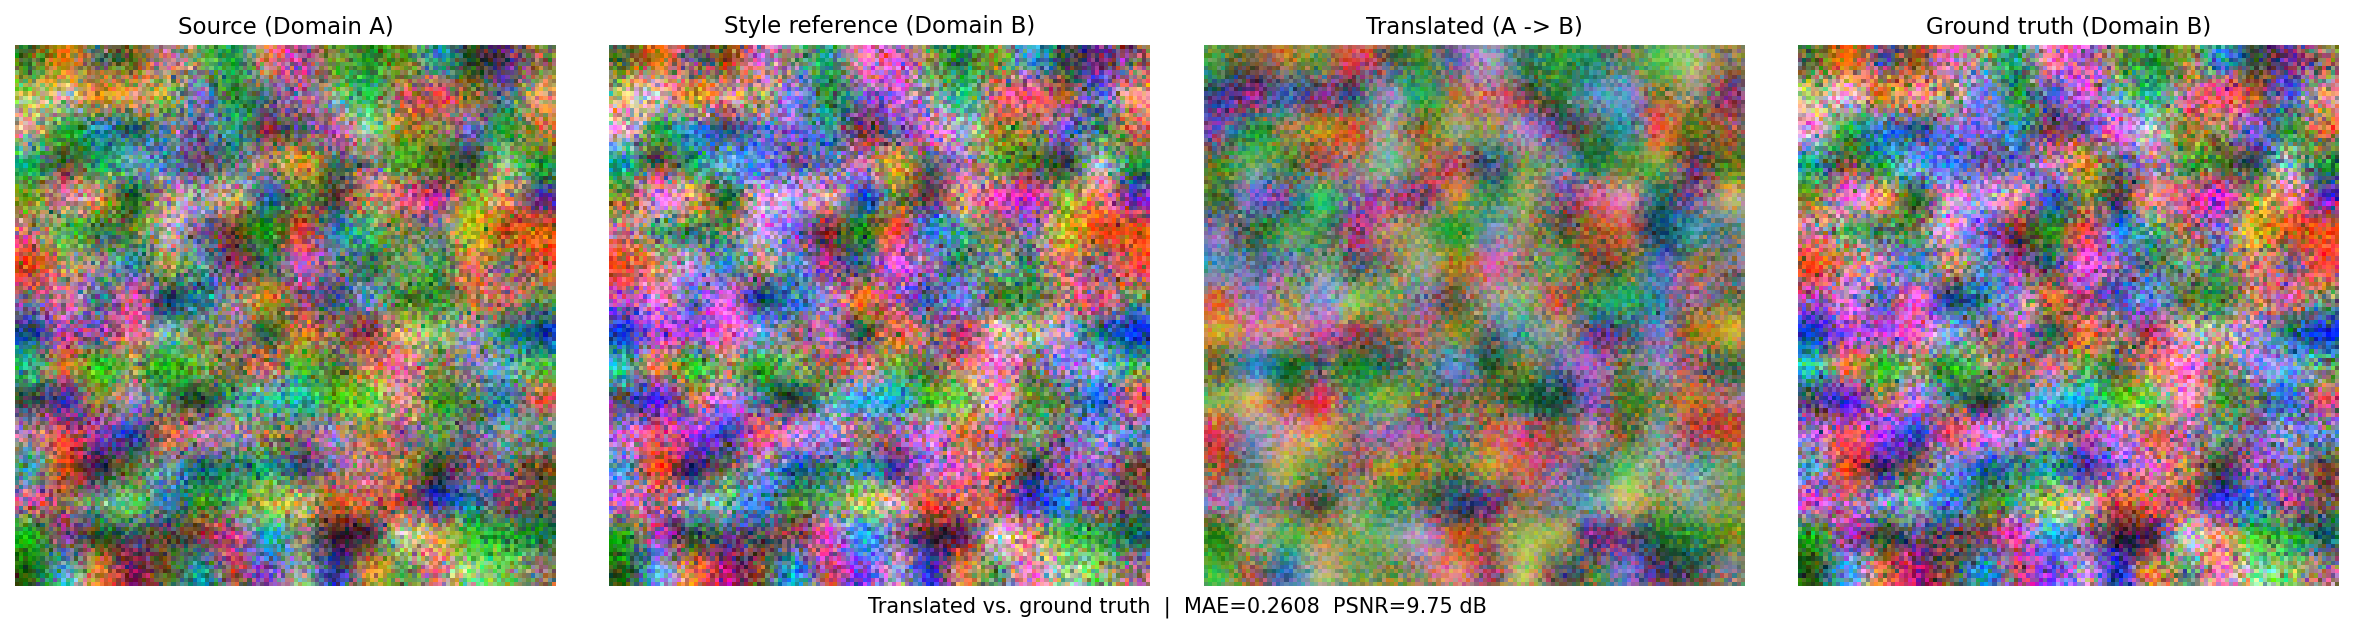
\includegraphics[width=0.95\textwidth]{translation_result.png}
    \caption{Qualitative comparison: source (domain A), the
             brightness-matched style reference (domain B), the
             translated output, and the paired ground truth. Images are
             a crude RGB preview of the packed RGGB tensors (averaged
             green channels), not a real demosaic.}
\end{figure}

% =====================================================================
\section{Discussion and Limitations}
% =====================================================================

\begin{itemize}[nosep]
    \item \textbf{Synthetic data only.} The demo's ``scenes'' are smooth
          random fields, not real photographic content -- there is no
          texture, edges, or objects for the model to preserve, so the
          translation problem is considerably easier than on real
          camera images. Results here should not be interpreted as
          evidence of photorealistic RAW2RAW quality.
    \item \textbf{No adversarial or noise-matching loss.} Because
          $\mathcal{L}_{\text{adv}}$ and $\mathcal{L}_{\text{noise}}$ are
          omitted, the demo cannot claim to reproduce the paper's central
          contribution (explicit sensor-noise-statistics alignment) --
          it only reproduces the style-conditioning and cycle-consistency
          mechanism.
    \item \textbf{No real transformer components.} The style encoder and
          generator bottleneck use plain convolutions rather than the
          self-attention blocks specified in Fig.~2 of the paper (see
          Table~\ref{sec:arch-deviations}).
    \item \textbf{Two domains only.} The paper's main scalability claim
          (near-constant parameter count/training cost as domain count
          grows from 3 to 5, Table~5 of \cite{merit2026}) is not
          exercised here, since only two synthetic domains are used.
    \item \textbf{Cycle+style losses alone do not guarantee improved
          paired-ground-truth fidelity.} As reported in
          Sec.~\ref{sec:training-run}, training loss decreased steadily,
          but MAE/PSNR against a held-out paired ground truth got
          \emph{worse}, not better, over training (Table~\ref{tab:results}). This
          empirically confirms that $\mathcal{L}_{\text{cycle}}$ and
          $\mathcal{L}_{\text{style}}$ alone are insufficient to
          reproduce the paper's reported translation quality -- the
          omitted adversarial and noise losses appear to be necessary,
          not merely beneficial, for grounding outputs in the target
          domain's realistic distribution.
\end{itemize}

% =====================================================================
\section{Conclusion}
% =====================================================================

This project implements a reduced-scale but functionally faithful
version of MERIT's style-conditioned translation mechanism: a
content-independent style encoder, a style-modulated MS-LKA generator,
unpaired cycle-consistency training, brightness-based reference
selection at inference, and the paper's own four-metric evaluation
protocol. The main simplifications relative to the full paper are the
omission of the adversarial and sensor-noise losses, the use of plain
convolutions in place of the paper's transformer blocks, and the use of
synthetic rather than real multi-camera RAW data.

The training run reported in Sec.~\ref{sec:training-run}--\ref{sec:deviations}
also produced an instructive negative result: while the training loss
itself converged smoothly, MAE/PSNR against a paired ground truth did
not improve over training, and in fact regressed relative to an
untrained baseline. Taken together with the architecture and loss
deviations catalogued in this report, this suggests that MERIT's
reported translation quality depends materially on components this demo
omits -- particularly the adversarial loss (which anchors outputs to
the realistic target-domain distribution) and the sensor-aware noise
loss (which explicitly aligns noise statistics with the target domain)
-- rather than on the style-conditioning and cycle-consistency mechanism
alone. A natural next step would be to add a minimal discriminator and
$\mathcal{L}_{\text{noise}}$ term to this same codebase and check
whether paired-ground-truth MAE/PSNR then improves with training, which
would directly test this hypothesis.

% =====================================================================
\bibliographystyle{plain}
\begin{thebibliography}{9}

\bibitem{merit2026}
Wenjun Huang, Shenghao Fu, Yian Jin, Yang Ni, Ziteng Cui, Hanning Chen,
Yirui He, Yezi Liu, Sanggeon Yun, SungHeon Jeong, Ryozo Masukawa,
William Youngwoo Chung, Mohsen Imani.
\emph{MERIT: Multi-domain Efficient RAW Image Translation}.
arXiv:2603.20836, 2026.

\bibitem{afifi2021}
Mahmoud Afifi and Abdullah Abuolaim.
\emph{Semi-supervised raw-to-raw mapping}.
arXiv:2106.13883, 2021.

\end{thebibliography}

% =====================================================================
\appendix
\section{Full Source Code}

\subsection{data\_generator.py}
\lstinputlisting[style=pystyle]{../src/data_generator.py}

\subsection{data\_preprocessing.py}
\lstinputlisting[style=pystyle]{../src/data_preprocessing.py}

\subsection{model.py}
\lstinputlisting[style=pystyle]{../src/model.py}

\subsection{train.py}
\lstinputlisting[style=pystyle]{../src/train.py}

\subsection{evaluate.py}
\lstinputlisting[style=pystyle]{../src/evaluate.py}

\subsection{main.py}
\lstinputlisting[style=pystyle]{../src/main.py}

\end{document}